\documentclass[]{article}
\usepackage[T1]{fontenc}
\usepackage{lmodern}
\usepackage{amssymb,amsmath}
\usepackage{ifxetex,ifluatex}
\usepackage{fixltx2e} % provides \textsubscript
% use upquote if available, for straight quotes in verbatim environments
\IfFileExists{upquote.sty}{\usepackage{upquote}}{}
\ifnum 0\ifxetex 1\fi\ifluatex 1\fi=0 % if pdftex
  \usepackage[utf8]{inputenc}
\else % if luatex or xelatex
  \ifxetex
    \usepackage{mathspec}
    \usepackage{xltxtra,xunicode}
  \else
    \usepackage{fontspec}
  \fi
  \defaultfontfeatures{Mapping=tex-text,Scale=MatchLowercase}
  \newcommand{\euro}{€}
\fi
% use microtype if available
\IfFileExists{microtype.sty}{\usepackage{microtype}}{}
\usepackage[margin=1in]{geometry}
\usepackage{color}
\usepackage{fancyvrb}
\newcommand{\VerbBar}{|}
\newcommand{\VERB}{\Verb[commandchars=\\\{\}]}
\DefineVerbatimEnvironment{Highlighting}{Verbatim}{commandchars=\\\{\}}
% Add ',fontsize=\small' for more characters per line
\usepackage{framed}
\definecolor{shadecolor}{RGB}{248,248,248}
\newenvironment{Shaded}{\begin{snugshade}}{\end{snugshade}}
\newcommand{\KeywordTok}[1]{\textcolor[rgb]{0.13,0.29,0.53}{\textbf{{#1}}}}
\newcommand{\DataTypeTok}[1]{\textcolor[rgb]{0.13,0.29,0.53}{{#1}}}
\newcommand{\DecValTok}[1]{\textcolor[rgb]{0.00,0.00,0.81}{{#1}}}
\newcommand{\BaseNTok}[1]{\textcolor[rgb]{0.00,0.00,0.81}{{#1}}}
\newcommand{\FloatTok}[1]{\textcolor[rgb]{0.00,0.00,0.81}{{#1}}}
\newcommand{\CharTok}[1]{\textcolor[rgb]{0.31,0.60,0.02}{{#1}}}
\newcommand{\StringTok}[1]{\textcolor[rgb]{0.31,0.60,0.02}{{#1}}}
\newcommand{\CommentTok}[1]{\textcolor[rgb]{0.56,0.35,0.01}{\textit{{#1}}}}
\newcommand{\OtherTok}[1]{\textcolor[rgb]{0.56,0.35,0.01}{{#1}}}
\newcommand{\AlertTok}[1]{\textcolor[rgb]{0.94,0.16,0.16}{{#1}}}
\newcommand{\FunctionTok}[1]{\textcolor[rgb]{0.00,0.00,0.00}{{#1}}}
\newcommand{\RegionMarkerTok}[1]{{#1}}
\newcommand{\ErrorTok}[1]{\textbf{{#1}}}
\newcommand{\NormalTok}[1]{{#1}}
\usepackage{longtable,booktabs}
\usepackage{graphicx}
% Redefine \includegraphics so that, unless explicit options are
% given, the image width will not exceed the width of the page.
% Images get their normal width if they fit onto the page, but
% are scaled down if they would overflow the margins.
\makeatletter
\def\ScaleIfNeeded{%
  \ifdim\Gin@nat@width>\linewidth
    \linewidth
  \else
    \Gin@nat@width
  \fi
}
\makeatother
\let\Oldincludegraphics\includegraphics
{%
 \catcode`\@=11\relax%
 \gdef\includegraphics{\@ifnextchar[{\Oldincludegraphics}{\Oldincludegraphics[width=\ScaleIfNeeded]}}%
}%
\ifxetex
  \usepackage[setpagesize=false, % page size defined by xetex
              unicode=false, % unicode breaks when used with xetex
              xetex]{hyperref}
\else
  \usepackage[unicode=true]{hyperref}
\fi
\hypersetup{breaklinks=true,
            bookmarks=true,
            pdfauthor={},
            pdftitle={},
            colorlinks=true,
            citecolor=blue,
            urlcolor=blue,
            linkcolor=magenta,
            pdfborder={0 0 0}}
\urlstyle{same}  % don't use monospace font for urls
\setlength{\parindent}{0pt}
\setlength{\parskip}{6pt plus 2pt minus 1pt}
\setlength{\emergencystretch}{3em}  % prevent overfull lines
\setcounter{secnumdepth}{5}

\author{}
\date{}

\begin{document}

\begin{center}
\normalsize
\end{center}


{
\hypersetup{linkcolor=black}
\setcounter{tocdepth}{2}
\tableofcontents
}
\section{Reproducible Research: Peer Assessment
1}\label{reproducible-research-peer-assessment-1}

by Melinda Higgins dated 07/09/2014

\subsection{Loading and preprocessing the
data}\label{loading-and-preprocessing-the-data}

\begin{Shaded}
\begin{Highlighting}[]
\CommentTok{# The following code assumes a relative path where the data are located in a subdirectory called "/data/"}
\NormalTok{activityData <-}\StringTok{ }\KeywordTok{read.csv}\NormalTok{(}\StringTok{"data/activity.csv"}\NormalTok{, }\DataTypeTok{header=}\OtherTok{TRUE}\NormalTok{)}
\end{Highlighting}
\end{Shaded}

\subsubsection{Summary of the dataset}\label{summary-of-the-dataset}

The data contain 3 columns of data which are " steps, date, interval ``.

There are 17568 rows of data covering 61 days. Each day the number of
steps were recorded every 5 minutes during 24 hours for 288 total
intervals per day.

\subsubsection{Missing data, Zeros, and Potential Extreme Values
(Potential
Outliers)}\label{missing-data-zeros-and-potential-extreme-values-potential-outliers}

\begin{itemize}
\itemsep1pt\parskip0pt\parsep0pt
\item
  There are 2304 NA's (missing values);
\item
  There are 11014 zeros (0's);
\item
  and 4250 entries with non-zero steps ranging from 1 to 806 steps in
  the 5 minute intervals.
\end{itemize}

Some of these high values seem extreme - possibly too many steps
recorded in a 5 minute interval. For example, the maximum number of
steps of 806 in 5 minutes implies making 2.6867 steps every second.

\subsubsection{Histogram of the Number of Steps Per 5 minute Interval
(ignoring missing
data)}\label{histogram-of-the-number-of-steps-per-5-minute-interval-ignoring-missing-data}

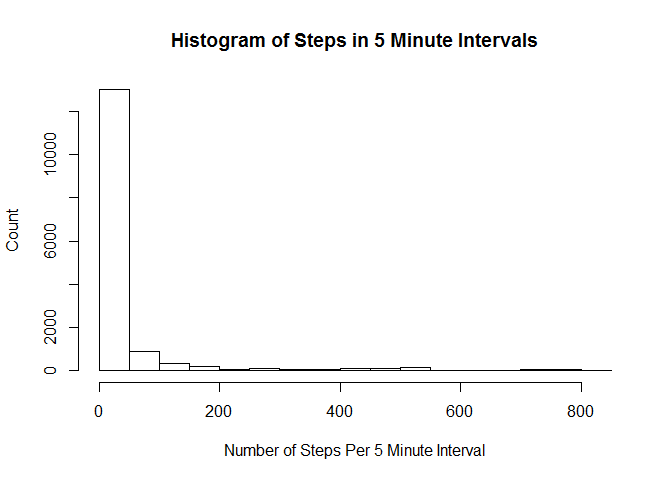
\includegraphics{./PA1_template_files/figure-latex/hist11.pdf}
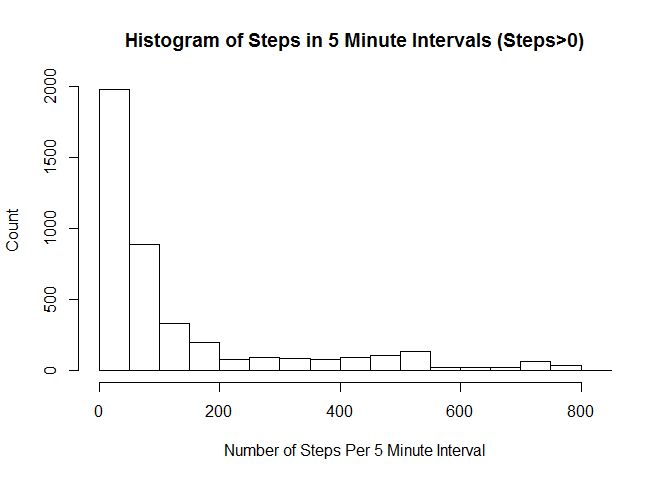
\includegraphics{./PA1_template_files/figure-latex/hist12.pdf}

\subsection{What is mean total number of steps taken per
day?}\label{what-is-mean-total-number-of-steps-taken-per-day}

Calculate the overall mean and the mean for each day. Also run for the
medians per day and overall - with an without the ``imputation'' method
tried below\ldots{}

\subsection{What is the average daily activity
pattern?}\label{what-is-the-average-daily-activity-pattern}

Look at the raw data - scatterplot by time of day (the increments) -
look at overall and by day of the week - also look at a table
summarizing these data given the n, mean, median, maybe Q1, Q3, min and
max - over all 61 days by time of day and again by day of week. make
some plots to go along with\ldots{}

\begin{Shaded}
\begin{Highlighting}[]
\KeywordTok{library}\NormalTok{(chron)}
\KeywordTok{library}\NormalTok{(lattice)}

\NormalTok{activitydate <-}\StringTok{ }\KeywordTok{chron}\NormalTok{(}\KeywordTok{as.character}\NormalTok{(activityData$date),}\DataTypeTok{format=}\KeywordTok{c}\NormalTok{(}\DataTypeTok{dates=}\StringTok{"y-m-d"}\NormalTok{),}\DataTypeTok{out.format=}\KeywordTok{c}\NormalTok{(}\StringTok{"day months year"}\NormalTok{))}

\NormalTok{activityData2 <-}\StringTok{ }\NormalTok{activityData}
\NormalTok{activityData2$date2 <-}\StringTok{ }\NormalTok{activitydate}
\NormalTok{activityData2$weekday <-}\StringTok{ }\KeywordTok{weekdays}\NormalTok{(activityData2$date2)}

\KeywordTok{library}\NormalTok{(xtable)}

\NormalTok{testdataf <-}\StringTok{ }\NormalTok{activityData2[}\DecValTok{1}\NormalTok{:}\DecValTok{30}\NormalTok{,]}
\NormalTok{testdataf.xtable <-}\StringTok{ }\KeywordTok{xtable}\NormalTok{(activityData2[}\DecValTok{1}\NormalTok{:}\DecValTok{30}\NormalTok{,])}
\KeywordTok{print}\NormalTok{(testdataf.xtable, }\DataTypeTok{floating=}\OtherTok{FALSE}\NormalTok{)}
\end{Highlighting}
\end{Shaded}

\begin{verbatim}
## Warning: class of 'x' was discarded
\end{verbatim}

\begin{verbatim}
## % latex table generated in R 3.1.0 by xtable 1.7-3 package
## % Sat Jul 12 11:52:05 2014
## \begin{tabular}{rrlrrl}
##   \hline
##  & steps & date & interval & date2 & weekday \\ 
##   \hline
## 1 &  & 2012-10-01 &   0 & 15614.00 & Mon \\ 
##   2 &  & 2012-10-01 &   5 & 15614.00 & Mon \\ 
##   3 &  & 2012-10-01 &  10 & 15614.00 & Mon \\ 
##   4 &  & 2012-10-01 &  15 & 15614.00 & Mon \\ 
##   5 &  & 2012-10-01 &  20 & 15614.00 & Mon \\ 
##   6 &  & 2012-10-01 &  25 & 15614.00 & Mon \\ 
##   7 &  & 2012-10-01 &  30 & 15614.00 & Mon \\ 
##   8 &  & 2012-10-01 &  35 & 15614.00 & Mon \\ 
##   9 &  & 2012-10-01 &  40 & 15614.00 & Mon \\ 
##   10 &  & 2012-10-01 &  45 & 15614.00 & Mon \\ 
##   11 &  & 2012-10-01 &  50 & 15614.00 & Mon \\ 
##   12 &  & 2012-10-01 &  55 & 15614.00 & Mon \\ 
##   13 &  & 2012-10-01 & 100 & 15614.00 & Mon \\ 
##   14 &  & 2012-10-01 & 105 & 15614.00 & Mon \\ 
##   15 &  & 2012-10-01 & 110 & 15614.00 & Mon \\ 
##   16 &  & 2012-10-01 & 115 & 15614.00 & Mon \\ 
##   17 &  & 2012-10-01 & 120 & 15614.00 & Mon \\ 
##   18 &  & 2012-10-01 & 125 & 15614.00 & Mon \\ 
##   19 &  & 2012-10-01 & 130 & 15614.00 & Mon \\ 
##   20 &  & 2012-10-01 & 135 & 15614.00 & Mon \\ 
##   21 &  & 2012-10-01 & 140 & 15614.00 & Mon \\ 
##   22 &  & 2012-10-01 & 145 & 15614.00 & Mon \\ 
##   23 &  & 2012-10-01 & 150 & 15614.00 & Mon \\ 
##   24 &  & 2012-10-01 & 155 & 15614.00 & Mon \\ 
##   25 &  & 2012-10-01 & 200 & 15614.00 & Mon \\ 
##   26 &  & 2012-10-01 & 205 & 15614.00 & Mon \\ 
##   27 &  & 2012-10-01 & 210 & 15614.00 & Mon \\ 
##   28 &  & 2012-10-01 & 215 & 15614.00 & Mon \\ 
##   29 &  & 2012-10-01 & 220 & 15614.00 & Mon \\ 
##   30 &  & 2012-10-01 & 225 & 15614.00 & Mon \\ 
##    \hline
## \end{tabular}
\end{verbatim}

\begin{Shaded}
\begin{Highlighting}[]
\KeywordTok{xyplot}\NormalTok{(activityData2$steps ~}\StringTok{ }\NormalTok{activityData2$interval |}\StringTok{ }\KeywordTok{factor}\NormalTok{(activityData2$weekday), }\DataTypeTok{type=}\KeywordTok{c}\NormalTok{(}\StringTok{"p"}\NormalTok{,}\StringTok{"spline"}\NormalTok{),}\DataTypeTok{col.line=}\StringTok{"darkorange"}\NormalTok{,}\DataTypeTok{lwd=}\DecValTok{3}\NormalTok{, }\DataTypeTok{layout=}\KeywordTok{c}\NormalTok{(}\DecValTok{1}\NormalTok{,}\DecValTok{7}\NormalTok{))}
\end{Highlighting}
\end{Shaded}

\begin{figure}[htbp]
\centering
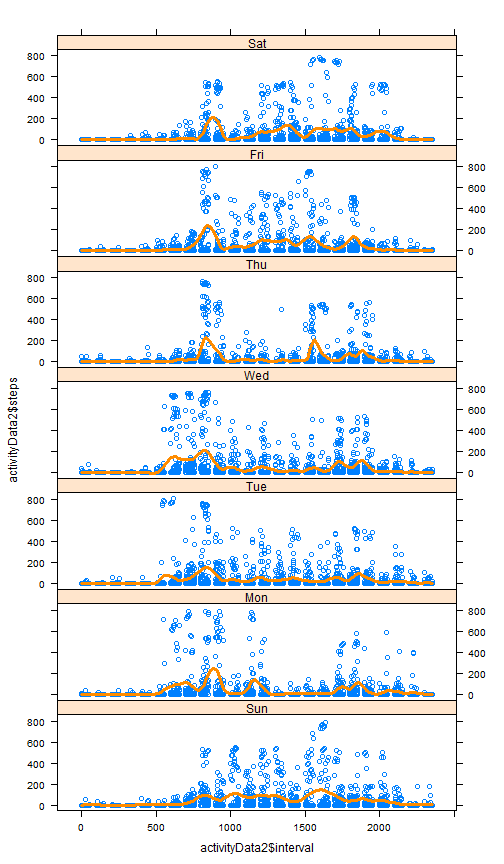
\includegraphics{./PA1_template_files/figure-latex/extractdates.pdf}
\caption{plot of chunk extractdates}
\end{figure}

Estimate

Std. Error

t value

Pr(\textgreater{}\textbar{}t\textbar{})

(Intercept)

29.5539

1.7868

16.54

0.0000

activityData2\$interval

0.0066

0.0013

5.08

0.0000

\subsubsection{Summary Statistics for Number of Steps in 5 Minute
Intervals}\label{summary-statistics-for-number-of-steps-in-5-minute-intervals}

sumsteps

0

3

12

1

37.4

1

806

1

2304

1

\section{\#\#\# Summary Statistics for Number of Steps (in 5 min
interval)}\label{summary-statistics-for-number-of-steps-in-5-min-interval}

\begin{longtable}[c]{@{}lr@{}}
\toprule\addlinespace
Statistic & Value
\\\addlinespace
\midrule\endhead
Mean & 37.38
\\\addlinespace
Median & 0
\\\addlinespace
SD & 112
\\\addlinespace
Min & 0
\\\addlinespace
Max & 806
\\\addlinespace
\bottomrule
\end{longtable}

\subsection{Imputing missing values}\label{imputing-missing-values}

Need to consider why the data are ``missing'' (NA's). These are most
likely due to inactivity, although zeros were also recorded during other
entries. Perhaps the NAs are due to the monitor being turned off or
other reason no data was recorded.

If we assume that the NA's are due to inactivity then substituting 0's
for NA would be appropriate. If this cannot be confirmed, a smoothing
approach could be used taking a simple average of the reading before and
after the NA is noted. Although if the reading before and after are both
NAs then perhaps a zero is best.

However, the number of steps are highly right-skewed with obvious
zero-inflation. This distribution indicates that using the mean to
substitute for the NAs is not appropriate. Instead using the median
would be better - although these are essentially zero for every day as
well - again suggesting that substituting zero's for the NAs would be
appropriate.

It is noted that without a proper explanation for the source of the NAs,
any method used for substitution will be biased. To what extent the
chosen method is biased is unverifiable without further information.

\subsection{Are there differences in activity patterns between weekdays
and
weekends?}\label{are-there-differences-in-activity-patterns-between-weekdays-and-weekends}

Need to figure out what function is needed to extract day of the week
from the provided dates. Also need to check the date formatting\ldots{}

\end{document}
